\section{Analysis and Opportunities for a Video Streaming Architecture}
\label{sec:system-archi}

%{\color{blue} This section explains the architecture system, and what it is for, explaining some protocols flowcharts. Studying the protocols and focusing in the system part of the experiments.}

%This section explains the modeling used in our experiments. We first provide an overview of the proposed video streaming service impacts in multi-tier networks. The remaining subsections describe the implementation of this service architecture.
Designing a cache hierarchy on vertically organized edge nodes with an arbitrary number of tiers can present improvements in users’ QoE~\cite{rana2018vertical}. The architecture mentioned above works toward such advantages by serving the requested content as close as possible to the end-user, efficiently forwarding requests between parent edge nodes within the hierarchy, and balancing the video traffic considering hop counts and users attended. In addition, the network core congestion is reduced since it represents an operational overhead for the content provider.
As a preliminary outcome achieved by a multi-tier network experiment, the QoE impact over a video streaming service is assessed. After that, we describe some results about the QoE characteristics and insights on the opportunities of caching multimedia content in edge nodes of multi-tier networks.

\subsection{Impact of Fog Multi-tier Network Approach}

To illustrate the differences in users' performance requesting a video from cache nodes in different tiers, consider two users requesting the same multimedia content from different layers. Then, an analysis of the impacts over the network is performed. Figure~\ref{fig:impact-two-layers} illustrates a two-tier network model. The graphs show the results of bitrate, interruptions (stalls), video buffer, and representations switch, respectively, from left to right.%and along x-axis the simulation time. 
\begin{figure*}[htp!]
    \centering
    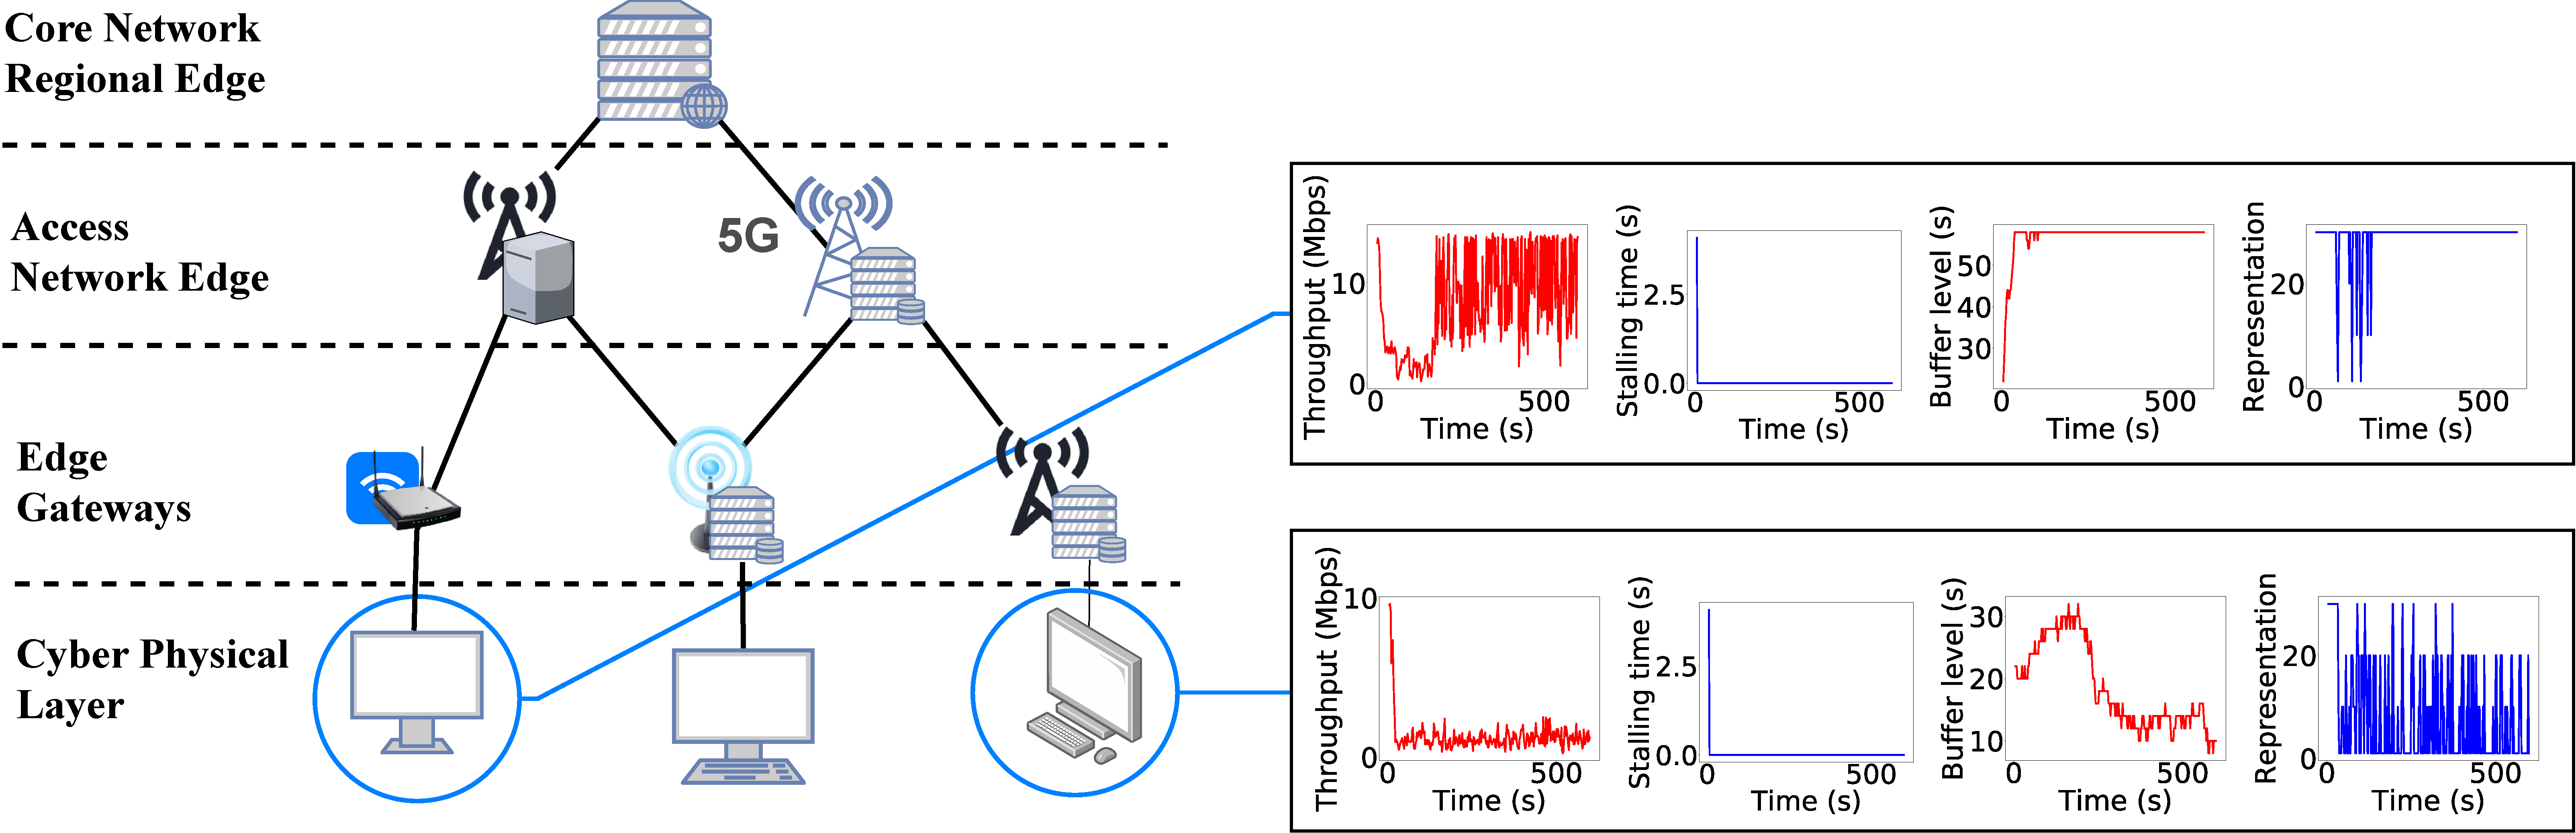
\includegraphics[width=\linewidth]{images/qoe-multi-level-3.pdf}
    \caption{Bitrate switches, stalls, buffer size, the startup delay in seconds of a DASH player was requesting a video with 10 bitrate levels varying from 50 to 4,500Kbps and from nodes in different tiers.}
    \label{fig:impact-two-layers}
\end{figure*}
Although a user requests a cache edge node video, it can be located in layers L1 or L2. Each layer level has different network factors, e.g., load, latency, so on. In Figure~\ref{fig:multi-tier-network}, an L1 layer can be interpreted as a personal computer, Access Point or Base Station, and this layer transmits the video content through wired or wireless communication channels, whereas in the L2 layer, a specific Edge gateway can be distributed on local edge nodes.

Apart from the initial interruption before the start of the video, both users did not experience the same issue again during the video execution. However, the user who received the video from the nearest edge layer had a higher bit rate than the user receiving the video from the upmost layer.
Note that the user receiving the video from the closest layer has filled the buffer faster, and thus he/she managed to keep the video playing at the best possible resolution.
On the other hand, the user who received the video from a more distant layer worked with the buffer at the limit and constantly switched resolutions so that there was no interruption during the video execution. Even without any interruptions in both video playbacks, the transmission from different tiers directly impacts the users' QoE.


\subsection{Multi-tier Edge-Cloud Network Opportunities}

%Esta seção apresenta algumas oportunidades dentro de redes multi-tier edge/cloud para o provisionamento da transmissção de videos. Aproveitar nós próximos aos usuários podem melhorar o funcionamento do rede como um todo, aqui nós discutimos alguns insights que podem ser usados em favor dos stakeholders que utilizam a infraestrutura para transmissão de video. 
Below are discussed the opportunities for resource management in multi-tier edge/cloud networks to provide video transmission. The advantages of nodes closer to end-users can improve the functioning of the network as a whole. We discuss some insights that can be used in favor of network and provider admin in the infrastructure for video transmission.

\subsubsection{Improving the User's QoE}

%the cloud distributes the video content to the different levels of the edge. Depending the level which the video is cached the users' experience changes. The architecture is based on held the video distribution with QoE support. The work divides the edge into three layers, to guarantee coverage, storage, upload and download capacity. 
In a multi-tier environment composed of more than one-tier resource availability, the resources can host the video content near the end-users. This allows reducing latency and mitigating the load on the network core. The edge nodes are composed of specific resources combined to carry out the video transmission to integrate video streaming services in such communication environments. Within this context, integrating QoE feedback models inside the player raises an opportunity to improve the users' satisfaction. % at each network level.
The results reported in Figure~\ref{fig:impact-two-layers} suggest that it is possible to improve the users' satisfaction using the edge multi-tier network. Depending on the video service allocation level, it is possible to provide a smooth video playback even in an overloaded network. % the video smoothing variation between characteristics of the player changes.

\subsubsection{Potential Bandwidth Saving}

%Video Caching, Analytics, and Delivery at the Wireless Edge: A Survey and Future Directions
Videos streamed in higher quality increase the network bandwidth use. Consequently, provisioning from the Cloud will incur high communication expenses in the core network. 
The process of delivering part of the video along the network can significantly save bandwidth instead of sending the entire video to an edge server or by lowering the encoding quality of uninteresting portions of the video. Different delivery approaches can have different performances to reduce the uplink bandwidth use. 
Because of that, it is possible to contemplate an end-to-end design of video streaming, wherein the edge server adapts the video streams based on uplink and downlink bandwidth capacities. Additionally, new forms of video content are being generated today and may present opportunities for bandwidth saving and video services orchestration in edge-cloud infrastructures.


\subsubsection{Cacheability}

%Caching audio/video during peak hours ...
%Manage the QoE users refer to those services where the Controller can centrally control the satisfaction guarantees. The Controller can address this problem by creating a control channel to managed-quality video streaming services over the edge-cloud network.

Nodes located at the edge are responsible for providing resources to VoD providers to allocate their caches. 
The allocated caches make multi-hops within the edge itself to serve the end-user. 
With this characteristic, different possibilities in the multi-tier network still have to be studied, such as cache allocation, placement, replacement, and selection caches, usually making decisions in real-time. These problems can offer a better video streaming service. 
In addition, an orchestrator has to consider the user's mobility and/or the possibility of predicting the direction of movement. In this way, as the user changes their trajectory, new caching mechanisms can use this information to optimize streaming video services.
